%% Copyright 2019 Matheus H. J. Saldanha <mhjsaldanha@gmail.com>
%
% This work may be distributed and/or modified under the
% conditions of the LaTeX Project Public License, either version 1.3
% of this license or (at your option) any later version.
% The latest version of this license is in
%   http://www.latex-project.org/lppl.txt
% and version 1.3 or later is part of all distributions of LaTeX
% version 2005/12/01 or later.
%
% This work has the LPPL maintenance status `maintained'.

\documentclass[12pt,a4paper]{article}

% Pacotes para o português.
\usepackage[brazilian]{babel}
\usepackage[utf8]{inputenc}
\usepackage[T1]{fontenc}

\usepackage{graphicx}
\usepackage{xcolor}
\usepackage{indentfirst}
\usepackage{url}
\usepackage{array}
\usepackage[top=2cm, bottom=2cm, left=2cm, right=2cm]{geometry}
\usepackage{multirow}
\usepackage{amssymb}
\usepackage{amsmath}
\usepackage{caption}
\usepackage{setspace}
\usepackage{breakcites}
\usepackage{float}
\usepackage{times}
\usepackage{lipsum}

% Comando para marcar o texto para revisão.
\newcommand{\rev}[1]{\textcolor{red}{#1}}

% Permite escrever aspas normais "text" em vez de ``text''
\usepackage[autostyle]{csquotes}
\MakeOuterQuote{"}

\begin{document}

\doublespacing

\begin{titlepage}
    \begin{center}
        {\large \sc UNIVERSIDADE DE SÃO PAULO} \\
        {\large \sc INSTITUTO DE CIÊNCIAS MATEMÁTICAS E DE COMPUTAÇÃO}\\[0.7cm]
        {\small \sc DEPARTAMENTO DE SISTEMAS DE COMPUTAÇÃO}\\[2.8cm]

        % Título.
        {\large \sc Projeto de Pesquisa FAPESP}\\
        \rule{0.9\linewidth}{0.5mm} \\[0.4cm]
        {\large \bfseries Predição de Estruturas de Proteínas com Algoritmos Paralelos Ortogonais às Plataformas Paralelas}\\
        \rule{0.9\linewidth}{0.5mm} \\[0.4cm]
        {\small \sc Linha de Fomento: Bolsa no País - Regular - Iniciação Científica}\\[2.8cm]
    \end{center}
    
    % Assinaturas
    \begin{minipage}{0.45\textwidth}
        \emph{Candidato:}\\[2.08cm]
        \begin{picture}(5,20)(0,-22.5) 
            % \put(0,1){\includegraphics[scale=0.13]{figs/assinatura-aluno.jpg}}
            \put(0,0){\rule{0.9\linewidth}{0.5mm}}
            \put(0,-22.5){Matheus Henrique Junqueira Saldanha}
        \end{picture}
    \end{minipage}
    \hspace{1cm}
    \begin{minipage}{0.45\textwidth}
        \emph{Orientador:}\\[2.08cm]
        \begin{picture}(130,20)(0,-22.5)
            % \put(18,1){\includegraphics[scale=0.48]{figs/assinatura-orientador.png}}
            \put(0,0){\rule{0.9\linewidth}{0.5mm}}
            \put(0,-22.5){Paulo Sérgio Lopes de Souza}
        \end{picture}
    \end{minipage}

    \vfill

    % Data
    \begin{center}
        \makeatletter
        \@date
        \makeatother
    \end{center}
\end{titlepage}


\pagestyle{empty}
\begin{center}
    {\bf \Large Resumo}
\end{center}

Resumo do projeto. Deve haver no máximo 20 linhas como especificado em \url{http://www.fapesp.br/248#10}.


\noindent{}
\newpage
\pagestyle{empty}
\tableofcontents
\newpage
\setcounter{page}{1}
\pagestyle{plain}

\section{Introdução}
\label{section:introducao}

A FAPESP não estabelece normas rígidas quanto à formatação do projeto de iniciação científica. Ela especifica, no entanto, que deve haver no máximo 20 páginas escritas com espaçamento duplo. Para outras modalidades de bolsa, ela também expressa preferência por fonte \textit{Times New Roman}, ou semelhantes, em tamanho 12 pontos\footnote{Veja, por exemplo, \url{http://www.fapesp.br/10408}}.

\section{Problema da Predição de Estruturas de Proteínas}
\label{section:problemapsp}

Todas as informações dadas a seguir se referem ao que foi adotado no projeto submetido e aceito. Legendas de figuras ficam abaixo da figura (veja a Figura \ref{fig:aminosequence}). Legendas de tabelas ficam acima (veja Tabela \ref{tab:cronograma}).

Figuras podem ser justapostas, e cada figura recebe sua própria legenda, como visto nas Figuras \ref{fig:aminosequence} e \ref{fig:peptidebond}. No entanto, posicioná-las corretamente não é simples, então cuidado deve ser tomado. Em especial, atenção com os caracteres "\%" posicionados no final de certas linhas no arquivo latex deste projeto, pois eles são importantes para o correto funcionamento do ambiente \textit{minipage}.

\begin{figure}[htb]
\centering
\begin{minipage}{.4\textwidth}
  \centering
  \vspace{1cm}
  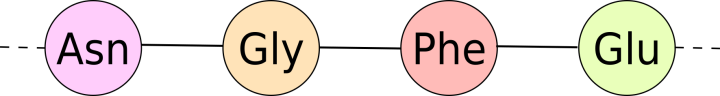
\includegraphics[width=0.8\textwidth]{imagens/amino_seq.png}
  \vspace{1cm}
  \captionof{figure}{Uma sequência dos aminoácidos: asparagina, glicina, fenilalanina e ácido glutâmico.}
  \label{fig:aminosequence}
\end{minipage}%
\hspace{.04\textwidth}%
\begin{minipage}{.55\textwidth}
  \centering
  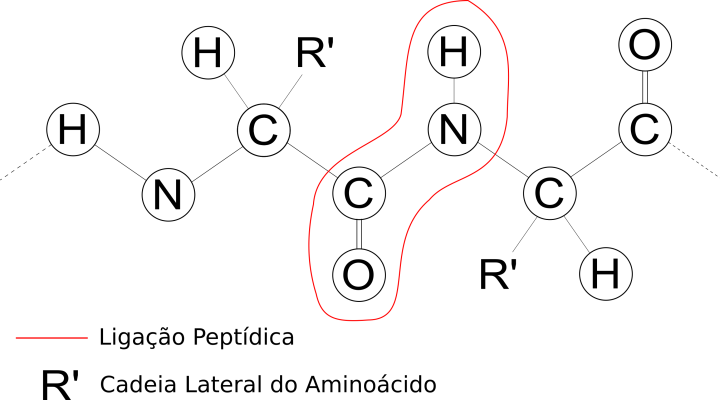
\includegraphics[width=0.8\linewidth]{imagens/protein_planar_pepbond.png}
  \captionof{figure}{Dois aminoácidos ligados por uma ligação peptídica.}
  \label{fig:peptidebond}
\end{minipage}
\end{figure}

Figuras retiradas de fontes externas devem ter sua fonte citada na legenda da mesma; caso contrário, poderia configurar plágio. Na Figura \ref{fig:hemoglobin3d}, a fonte é citada e uma URL é fornecida via nota de rodapé.

\begin{figure}[htb]
    \centering
    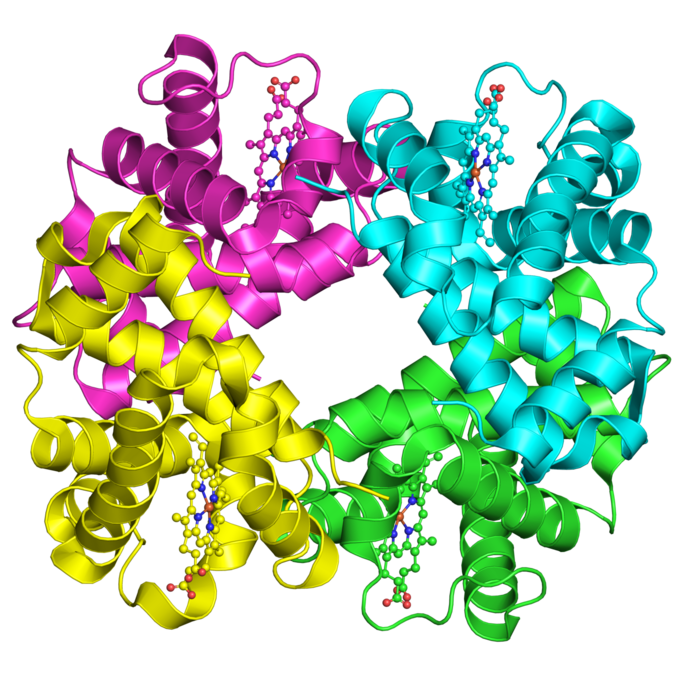
\includegraphics[width=0.35\linewidth]{imagens/3d_hemoglobin.png}
    \caption{Estrutura tridimensional da hemoglobina, obtida de \textit{Protein Data Bank in Europe} \protect\footnotemark{}.}
    \label{fig:hemoglobin3d}
\end{figure}

% Completa o \footnotemark utilizado na legenda da figura acima.
\footnotetext{https://www.ebi.ac.uk/pdbe/entry/pdb/1a3n}

Quando precisar de um pedaço qualquer de texto para preencher qualquer lugar temporariamente, pode-se usar o comando \textit{lipsum}, que resulta no parágrafo a seguir.

\lipsum[1]

Caso tenha algum parágrafo que precisa ser revisado futuramente, pode-se usar o comando \textit{rev}. Por exemplo, \rev{este texto precisa ser revisado}.

\section{Arquiteturas e Modelos de Programação Paralela}
\label{section:hpc}
Citações são essenciais para qualquer projeto de pesquisa. Por exemplo, no contexto de arquiteturas paralelas, uma boa referência é \cite{tanenbaum2016structured}. Para poder citar utilizando o comando \textit{cite}, preencha o arquivo \textit{bibliography.bib} com o devido registro no formato bibtex, que pode ser facilmente obtido em plataformas como o \textit{Google Scholar}.

Ressalta-se que a FAPESP não estabelece normas rígidas de formatação do projeto. Existem muitos pacotes latex interessantes que podem ser utilizados para embelezar o documento. Verifique, por exemplo, o pacote \textit{hyperref}, que pode ser utilizado para tornar links e referências internas (para figuras, tabelas, seções \textit{etc}) ``clicáveis'' e coloridos. Neste modelo, limitou-se a utilizar pacotes que foram utilizados no projeto submetido e aceito.

\section{Trabalhos Relacionados}
\label{section:trabrelacionados}
\input{text/trabrelacionados.tex}

\section{Objetivos}
\label{section:objetivos}
\input{text/objetivos.tex}

\section{Metodologia}
\label{section:metodologia}

A partir deste ponto, o conteúdo do projeto submetido e aceito é replicado, para ser tomado como base para a escrita da seção de metodologia.

\subsection{Atividades a Serem Desenvolvidas}
\label{section:atividadesdesenvolvidas}

A execução do projeto pode ser dividida nas seguintes etapas:

\begin{enumerate}
    \item \textbf{Seleção dos algoritmos}, quando algoritmos paralelos de predição de estruturas de proteínas, encontrados na literatura, serão selecionados, com suporte da engenharia reversa sobre os mesmos. Espera-se nesta etapa levantar não apenas quais algoritmos considerar para o desenvolvimento do projeto, mas também determinar seus principais requisitos com vistas a implementações paralelas em diferentes arquiteturas;
    
    \item \textbf{Reengenharia dos algoritmos selecionados}, quando a metodologia de projeto PCAM será aplicada aos algoritmos selecionados, instanciando-os aos modelos de programação considerados no projeto;
    
    \item \textbf{Implementação dos algoritmos}, na qual os algoritmos paralelos serão implementados e documentados, ao mesmo tempo que serão executados os testes de unidade durante a implementação para favorecer a confiabilidade do código final, diminuindo a possibilidade de defeitos não revelados nos códigos desenvolvidos;
    
    \item \textbf{Projeto e execução de experimentos}, quando experimentos serão projetados e executados visando validar os algoritmos implementados e obter os dados necessários para avaliar o desempenho dos mesmos (vide Seção \ref{section:analiseresultados} para maiores detalhes);

    \item \textbf{Finalização da documentação}, na qual será elaborada a documentação final do conjunto de algoritmos analisados e implementados, a ser disponibilizada publicamente para uso de outros pesquisadores. A disponibilização da documentação (em conjunto com os algoritmos implementados) ocorrerá na página do Laboratório de Sistemas Distribuídos e Programação Concorrente (LaSDPC) do ICMC/USP;
    
    \item \textbf{Redação de artigos científicos}, quando serão escritos artigos científicos descrevendo os resultados obtidos neste projeto de Iniciação Científica. Espera-se submeter artigos para o Simpósio em Sistemas Computacionais de Alto Desempenho (WSCAD) em 2018;
    
    \item \textbf{Redação dos Relatórios Científicos}, quando serão escritos os relatórios exigidos pelas normas da FAPESP.
    
\end{enumerate}

\subsection{Cronograma}

Com base nas tarefas enumeradas na Seção \ref{section:atividadesdesenvolvidas}, é mostrado na Tabela \ref{tab:cronograma} o cronograma a ser executado durante a realização deste projeto.

\begin{table}[ht]
\centering
\caption{Cronograma das atividades.}
\begin{tabular}{|c|c|c|c|c|c|c|c|c|c|c|c|c|}
\hline
\multirow{2}{*}{{\bf Fases}} & \multicolumn{12}{c|}{{\bf Meses}}
\\ \cline{2-13}
    & 1 & 2 & 3 & 4 & 5 & 6 & 7 & 8 & 9 & 10 & 11 & 12
\\ \hline
    {\bf 1. Seleção algoritmos} & x & x & & & & & & & & & &
\\ \hline
    {\bf 2. Reengenharia algoritmos} &  & x & x & & & & & & & & &
\\ \hline
    {\bf 3. Implementação algoritmos} & & x & x & x & x & x & x & & & & &
\\ \hline
    {\bf 4. Experimentos} & & & x & x & x & x & x & x & x & x &  & 
\\ \hline
    {\bf 5. Documentação} & & & & & & & & x & x & x & & 
\\ \hline
    {\bf 6. Artigos} &  &  &  &  &  &  &  &  & x & x & x & 
\\ \hline    
    {\bf 7. Relatórios} & & & & & x & x & & & & & x & x
\\ \hline
\end{tabular}
\label{tab:cronograma}
\end{table}


\subsection{Desafios Científicos e Técnicos}

% Não sei se entendi o conteúdo a ser escrito aqui.

\subsection{Material a Ser Utilizado}
\label{section:material}

\subsection{Forma de Análise dos Resultados}
\label{section:analiseresultados}


\begin{enumerate}
    \item eficiência e \textit{speedup} em relação à versão sequencial do mesmo algoritmo, variando-se a carga de trabalho (proteínas a serem preditas) e o tamanho da arquitetura sendo usada para a execução paralela;
    \item comparação da eficiência e \textit{speedups} obtidos pelos diferentes algoritmos, também variando-se as proteínas e as arquiteturas;
    \item menores energias calculadas, para cada dado de entrada e arquitetura utilizada.
\end{enumerate}

\begin{enumerate}
    % Número total de algoritmos
    \item devem ser implementados entre 4 e 8 algoritmos paralelos de predição de PSP. Este número foi estipulado em função dos algoritmos já encontrados na literatura em artigos científicos. Caso novos artigos sejam encontrados, seus algoritmos também serão considerados. Outrossim, acredita-se que a implementação dos algoritmos já descobertos seja possível; porém, isso será analisado em maior profundidade, de fato, durante o desenvolvimento do projeto, abrindo-se a possibilidade para que nem todos os algoritmos venham a ser codificados (por falta de informações e/ou retorno de seus autores, caso necessário);
    
    % Número de algoritmos algoritmos modificados que devo propor
    \item os algoritmos serão, tanto quanto possível, projetados visando execução em diferentes arquiteturas paralelas e codificação com diferentes modelos de programação.
\end{enumerate}

\subsection{Resultados Esperados}

\subsection{Exequibilidade}


\newpage

\bibliographystyle{apalike}
\bibliography{bibliography.bib}

\end{document}